\section{Results}
\paragraph{Reporting rule.}
Every value is imported from a versioned CSV artifact. Smoke tests establish compatibility only. The source-level selector audit below is a validation diagnostic used to freeze the routing protocol; VLM task, transfer, and selective-risk tables remain incomplete until the corresponding frozen runs finish.

\subsection{Dataset construction and shift}
Table~\ref{tab:data} records the audited data snapshot. Azalea is not a smaller copy of the Magnolia domain: it contains more labeled instances per source image but smaller normalized objects and a lower median green-pixel fraction (.312 versus .429). This measured shift defines the directed transfer experiment but does not itself establish robustness.

\paragraph{Effect of detector hard-negative mining.}
Table~\ref{tab:hnm} reports the matched validation comparison used to assess the detector refinement. One hard-negative mining round removed 101 false positives, an $11.6\%$ relative reduction, while AP$_{50{:}95}$ increased by $.011$. Precision and recall each increased by approximately $.006$. These changes indicate cleaner evidence entering OrnaScout; they are not attributed to the Budgeted Evidence Selector.

\begin{table}[t]
\centering
\wacvtablefont
\caption{Effect of one training-only hard-negative mining round on detector validation performance. Architecture, source split, optimization, augmentation, and evaluation settings are held fixed. False positives are measured by matching detections to validation annotations.}
\label{tab:hnm}
\setlength{\tabcolsep}{4.2pt}
\begin{tabular}{lrrrr}
\toprule
Detector training & AP$_{50{:}95}\uparrow$ & Prec.$\uparrow$ & Rec.$\uparrow$ & FP$\downarrow$ \\
\midrule
Baseline & .756 & .938 & .941 & 873 \\
+ one HNM round & \textbf{.767} & \textbf{.943} & \textbf{.947} & \textbf{772} \\
\bottomrule
\end{tabular}
\end{table}

\subsection{Selector ablation at equal budget}
Table~\ref{tab:selector} isolates the proposed selector using one primary VLM, fixed $K$, and identical decoding. The critical comparison is full exploit--explore routing against combined-score top-$K$: it tests whether reserved exploration contributes beyond detector ranking.
To isolate evidence allocation from gate fitting, AURC orders records with the fixed evidence score in Eq.~\eqref{eq:fixedgate}; no selector-specific threshold is fitted on the test set.

Before VLM inference, Table~\ref{tab:evidence-audit} tests whether each selector retains the annotated evidence at $B=8$. Count top-$K$ gives the highest evidence recall among deployable policies on validation ($.455$), narrowly ahead of combined top-$K$ ($.451$). Exploit--explore does not improve recall ($.439$), but reduces overlap redundancy and retains more hard-negative tiles than the detector-ranked policies. Spatially uniform selection attains similar recall with the broadest coverage and no tile overlap. These results prevent us from treating the proposed policy as uniformly superior; its value must be established by the downstream task and selective-risk experiments.

\begin{table}[t]
\centering
\wacvtablefont
\caption{Source-level validation audit at $B=8$. Evidence recall includes source-clustered 95\% CIs. GT oracle is diagnostic only.}
\label{tab:evidence-audit}
\setlength{\tabcolsep}{3.3pt}
\resizebox{\columnwidth}{!}{%
\begin{tabular}{lcccc}
\toprule
Selector & Evid. recall & Spatial cov. & Redund.$\downarrow$ & Hard-neg. rec. \\
\midrule
Random & $.352\;[.335,.382]$ & $.361$ & $.141$ & $.231$ \\
Spatial uniform & $.438\;[.415,.464]$ & $.411$ & $\mathbf{.000}$ & $.196$ \\
Confidence top-$K$ & $.384\;[.350,.425]$ & $.340$ & $.214$ & $.024$ \\
Count top-$K$ & $\mathbf{.455}\;[.420,.496]$ & $.330$ & $.252$ & $.015$ \\
Combined top-$K$ & $.451\;[.416,.494]$ & $.330$ & $.254$ & $.007$ \\
Exploit--explore & $.439\;[.410,.474]$ & $.345$ & $.196$ & $.067$ \\
Shuffled score & $.353\;[.336,.382]$ & $.361$ & $.142$ & $.236$ \\
GT oracle & $.506\;[.471,.544]$ & $.335$ & $.233$ & $.002$ \\
\bottomrule
\end{tabular}}
\end{table}

Figure~\ref{fig:selector-budget} reports the full budget sweep. Increasing $B$ predictably raises evidence recall and spatial coverage, but also increases redundant overlap. The curves are routing diagnostics, not VLM accuracy curves.

\begin{figure*}[t]
    \centering
    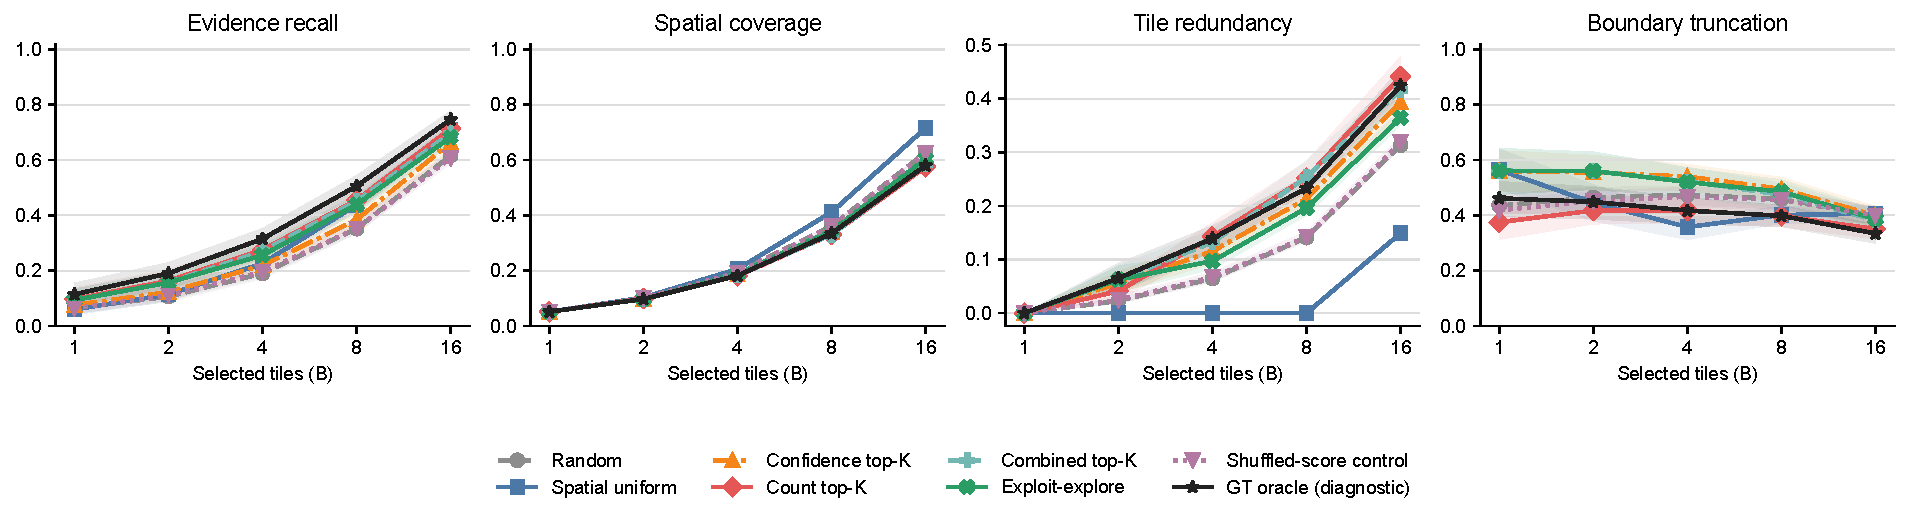
\includegraphics[width=\textwidth]{figures/selector_budget_audit_main.pdf}
    \caption{\textbf{Validation-only evidence audit across visual budgets.} Means and source-clustered 95\% bootstrap intervals are computed over 58 validation images. Random, exploit--explore, and shuffled-score policies are averaged over ten deterministic repetitions. The GT oracle uses annotations and is shown only to diagnose headroom.}
    \label{fig:selector-budget}
\end{figure*}

\begin{table}[t]
\centering
\wacvtablefont
\caption{Budgeted Evidence Selector ablation with SmolVLM2-2.2B at fixed $K=8$. Values are macro-F1 except AURC; brackets denote source-clustered 95\% bootstrap intervals.}
\label{tab:selector}
\setlength{\tabcolsep}{3.3pt}
\begin{tabular}{lccccc}
\toprule
Selector & Pres. & Count & Dens. & Cov. & AURC$\downarrow$\\
\midrule
Random & $0.465\;[0.447,0.481]$ & $0.003\;[0.000,0.008]$ & $0.000\;[0.000,0.000]$ & $0.230\;[0.220,0.238]$ & $1.000\;[1.000,1.000]$ \\
Spatial uniform & $0.466\;[0.451,0.479]$ & $0.005\;[0.000,0.012]$ & $0.000\;[0.000,0.000]$ & $0.232\;[0.224,0.238]$ & $1.000\;[1.000,1.000]$ \\
Confidence top-$K$ & $0.498\;[0.496,0.500]$ & $0.003\;[0.000,0.010]$ & $0.000\;[0.000,0.000]$ & $0.249\;[0.247,0.250]$ & $1.000\;[1.000,1.000]$ \\
Count top-$K$ & $0.500\;[0.500,0.500]$ & $0.011\;[0.001,0.024]$ & $0.000\;[0.000,0.000]$ & $0.250\;[0.249,0.250]$ & $1.000\;[1.000,1.000]$ \\
Combined top-$K$ & $0.500\;[0.500,0.500]$ & $0.013\;[0.001,0.029]$ & $0.000\;[0.000,0.000]$ & $0.250\;[0.250,0.250]$ & $1.000\;[1.000,1.000]$ \\
Exploit--explore & $0.492\;[0.487,0.496]$ & $0.011\;[0.001,0.024]$ & $0.000\;[0.000,0.000]$ & $0.246\;[0.243,0.248]$ & $1.000\;[1.000,1.000]$ \\
%
\end{tabular}
\end{table}

\subsection{VLM generality and efficiency}
Table~\ref{tab:models} holds selector, schema, and gate protocol fixed while changing the VLM. Report task macro-F1 as the unweighted mean of the four task F1 values. Edge orientation is determined from measured latency and memory.

\begin{table}[t]
\centering
\wacvtablefont
\caption{Model generality under the identical exploit--explore evidence budget ($K=8$, $\rho=.25$), prompt, schema, and generation length. Hall. is the false-positive rate on verified negative tiles; memory is peak resident or accelerator-reserved memory measured on the common evaluation device.}
\label{tab:models}
\setlength{\tabcolsep}{3pt}
\begin{tabular}{lccccc}
\toprule
Model & Macro-F1 & Schema & Hall.$\downarrow$ & p95 ms$\downarrow$ & GB$\downarrow$\\
\midrule
SmolVLM2-500M & $0.000$ & $0.000$ & $0.000$ & $61528$ & $2.84$ \\
SmolVLM2-2.2B & $0.187$ & $0.128$ & $1.000$ & $3536$ & $4.79$ \\
Phi-3.5-Vision & \tbd{pending} & \tbd{pending} & \tbd{pending} & \tbd{pending} & \tbd{pending} \\
LLaVA-1.5-7B & \tbd{pending} & \tbd{pending} & \tbd{pending} & \tbd{pending} & \tbd{pending} \\
%
\end{tabular}
\end{table}

\subsection{Cross-crop transfer}
Report M$\rightarrow$M, A$\rightarrow$A, M$\rightarrow$A, and A$\rightarrow$M separately as a $2\times2$ transfer matrix. The analysis must emphasize paired drops from each within-crop reference, with source-clustered intervals. Object scale and annotation density may be discussed as candidate mechanisms, not post-hoc proof.

\subsection{Selective reliability}
Risk--coverage curves compare raw VLM confidence, schema-only rejection, Eq.~\eqref{eq:fixedgate}, and the validation-fitted gate. Report coverage at a predeclared accepted-risk target, false-accept rate, and the number of accepted source clusters. Low risk at negligible coverage is not operationally useful.

\subsection{Failure analysis}
A balanced human-reviewed taxonomy distinguishes detector miss, boundary truncation, crop confusion, count-bin error, malformed schema, unsupported positive claim, and correct abstention. Qualitative panels show the selected evidence alongside the structured record and decision; examples are sampled by a frozen rule rather than chosen only for visual appeal.
